\documentclass[../main/main.tex]{subfiles}
\begin{document}

\setcounter{chapter}{3}
\chapter{\hypergal: Modéliseur de scène pour l'extraction de sources ponctuelles}\label{ch:hypergal}

\minitoc
\vspace{2cm}
La première partie de ce manuscrit était dédiée à la présentation du
contexte scientifique dans lequel ce travail de recherche est
effectué.

Nous avons dans un premier temps introduit les notions de
cosmologies nécessaires pour comprendre l'environnement scientifique de
travail, ainsi que la nature et le rôle des supernovae de type Ia en
tant que sondes cosmologiques.

Dans un second temps nous avons présenté la collaboration Zwicky
Transient Facility, ses différents groupes de recherches et plus
particulièrement la place qu'occupe l'étude des SNeIa dans ce relevé
astronomique nouvelle génération. 
Après avoir introduit la nécessité d'une méthode de
classification spectroscopique des évènements transitoires détectés par
la caméra ZTF, nous avons présenté la Spectral Energy Distribution
machine, un spectrographe 3D que possède la collaboration et
conçu pour la classification.

Le pipeline de réduction de données actuel, \pysedm, permet également une
extraction des sources ponctuelles observées par la caméra de l'IFU de
la SEDm. La méthode implémentée est toutefois rudimentaire, et ne permet
pas de palier aux nombreuses situations de contamination de la source
ponctuelle par sa galaxie hôte.

Non seulement cela induit une perte statistique de supernovae
classifiables non négligeable, mais de surcroît cela induit un biais
environnemental dans l'échantillon des SNeIa de ZTF.

C'est pour répondre à cette problématique que nous introduisons
\hypergal, un modéliseur de scène pour l'extraction de sources ponctuelles.

\newpage

\section{Idée générale}\label{sec:ideahypergal}

\subsection{Problématique}

Le champ de vue de la SEDm étant étroit ($28\times28\arcsec$), nous
avons en général $3$ composantes qui composent la
scène, à savoir le fond du ciel, la galaxie hôte et la source ponctuelle.

La difficulté majeure d'une modélisation de scène spectrale provient de la chromaticité de chacune de ces
composantes, et plus particulièrement de la galaxie qui est une source
structurée de forme et chromaticité variable.

Une première idée serait d'attendre l'extinction de l'évènement
transitoire, réobserver l'hôte, et projeter cette seconde acquisition
dans l'espace de la première observation afin d'isoler la source
ponctuelle. Une telle approche est envisageable pour une extraction de
quelques cibles, mais en aucun cas à notre époque où les relevés grands
champs et à haute cadence deviennent légions et observent des milliers
de supernovae par an.

Le but d'\hypergal est de pouvoir modéliser la scène observée
par la SEDm après réduction des données, c'est à dire le cube 3D, à la
volée des observations.

Il va donc non seulement falloir trouver un moyen de modéliser chacune
des composantes, mais également de les projeter dans l'espace des
observations de la SEDm. Cela implique une étude profonde des caractéristiques de
l'instrument mais également de prendre en compte les conditions
environnementales comme l'atmosphère le long de la ligne de visée.


\subsection{La composante galactique}

La motivation principale de ce modéliseur de scène est le fait que nous
avons des informations sur la galaxie hôte \underline{avant}
l'apparition de l'évènement transitoire. En effet, d'autres relevés
astronomiques comme le Sloan Digital Sky Survey (SDSS;
\citet{YorkSDSS2000}) ou Panstarrs \citep{ChambersPanstarrs} ont couvert
des portions communes de ciel avec ZTF, et permettent donc de remonter à
des informations photométriques de la galaxie encore isolée de la supernova.

Sauf que nous souhaitons une modélisation spectrale. Il faut donc un
moyen de passer de l'espace photométrique à l'espace spectral, autrement
dit estimer la Spectral Energy Distribution (SED) de la galaxie. 

Plus précisément encore, l'objectif est de pouvoir recréer un cube
3Dcontenant uniquement la galaxie, afin de pouvoir le projeter dans
l'espace de la SEDm en prenant en compte les propriétés de l'instrument et les
conditions d'observation. 
Donc non seulement il faut être en mesure de passer de l'espace
photométrique à l'espace spectral, mais il faut le faire localement pour
que chaque spaxel du cube modèle ait son propre spectre associé.

Une approche triviale de ce problème serait de partir d'images de
plusieurs bandes
photométriques de la galaxie, et interpoler un spectre pour chaque pixel
de ces images à l'aide d'un
simple polynome. Cela permettrait de créer un cube 3D avec une source structurée.
Mais grâce à l'avènement de nombreux instruments terrestres et spatiaux
lancés au cours des dernières décennies, nous avons une certaine
connaissance de la composition d'une galaxie, et ainsi des différentes
contributions qui forment sa SED.

L'idée est donc d'utiliser un SED Fitter appliqué aux données
photométriques de la galaxie, afin de construire un cube 3D qui servira de base pour le modéliseur de scène.

\section{SED Fitting}\label{sec:sedfitting}
\subsection{SED d'une galaxie}

Bien évidemment il est impossible de parler de SED Fitter sans parler
des connaissances existantes sur le spectre d'une galaxie.

Des rayons $\gamma$ au domaine radio, la SED d'une galaxie est définie par sa composition en matière
baryonique, et de leurs intéractions physiques complexes. En mettant de côté la matière
noire, une galaxie est composée d'étoiles de tout âge, de gaz atomiques
moléculaires ou ionisés, de poussières et
potentiellement d'un trou noir supermassif \citep{Kormendy}. Les étoiles
qui composent la galaxies (entre $10^{8}$ et $10^{14}$) émettent la
lumière qui nous permet de la détecter. D'autre part, le gaz interstellaire
et la poussière vont quant à eux principalement altérer la SED: le gaz en ajoutant des raies
d'émission et d'absorption, la poussière en provocant une atténuation par
absorption dans l'UV/proche infrarouge et une diffusion des radiations, puis en
ré-émettant dans l'infrarouge moyen/lointain.

L'état de ces composantes et
leurs intéractions nous renseignent sur les propriétés physiques fondamentales
de la galaxie: le taux de formation stellaire (SFR) et son histoire
(SFH), la masse stellaire, la metallicité, les propriétés d'atténuation, la masse de
poussière, les émissions nébulaires ou encore la présence possible d'un noyau actif (AGN). 

La SED d'une galaxie contient ainsi l'empreinte de tous ces ingrédients
et phénomènes physiques complexes, évoluants au cours du temps et traçant
l'histoire de la galaxie. Deux exemples de spectres de galaxies obtenus
avec le relevé SDSS dans l'optique sont
présentés dans la Figure~\ref{fig:specgalsdss}.

\begin{figure}
  \centering
  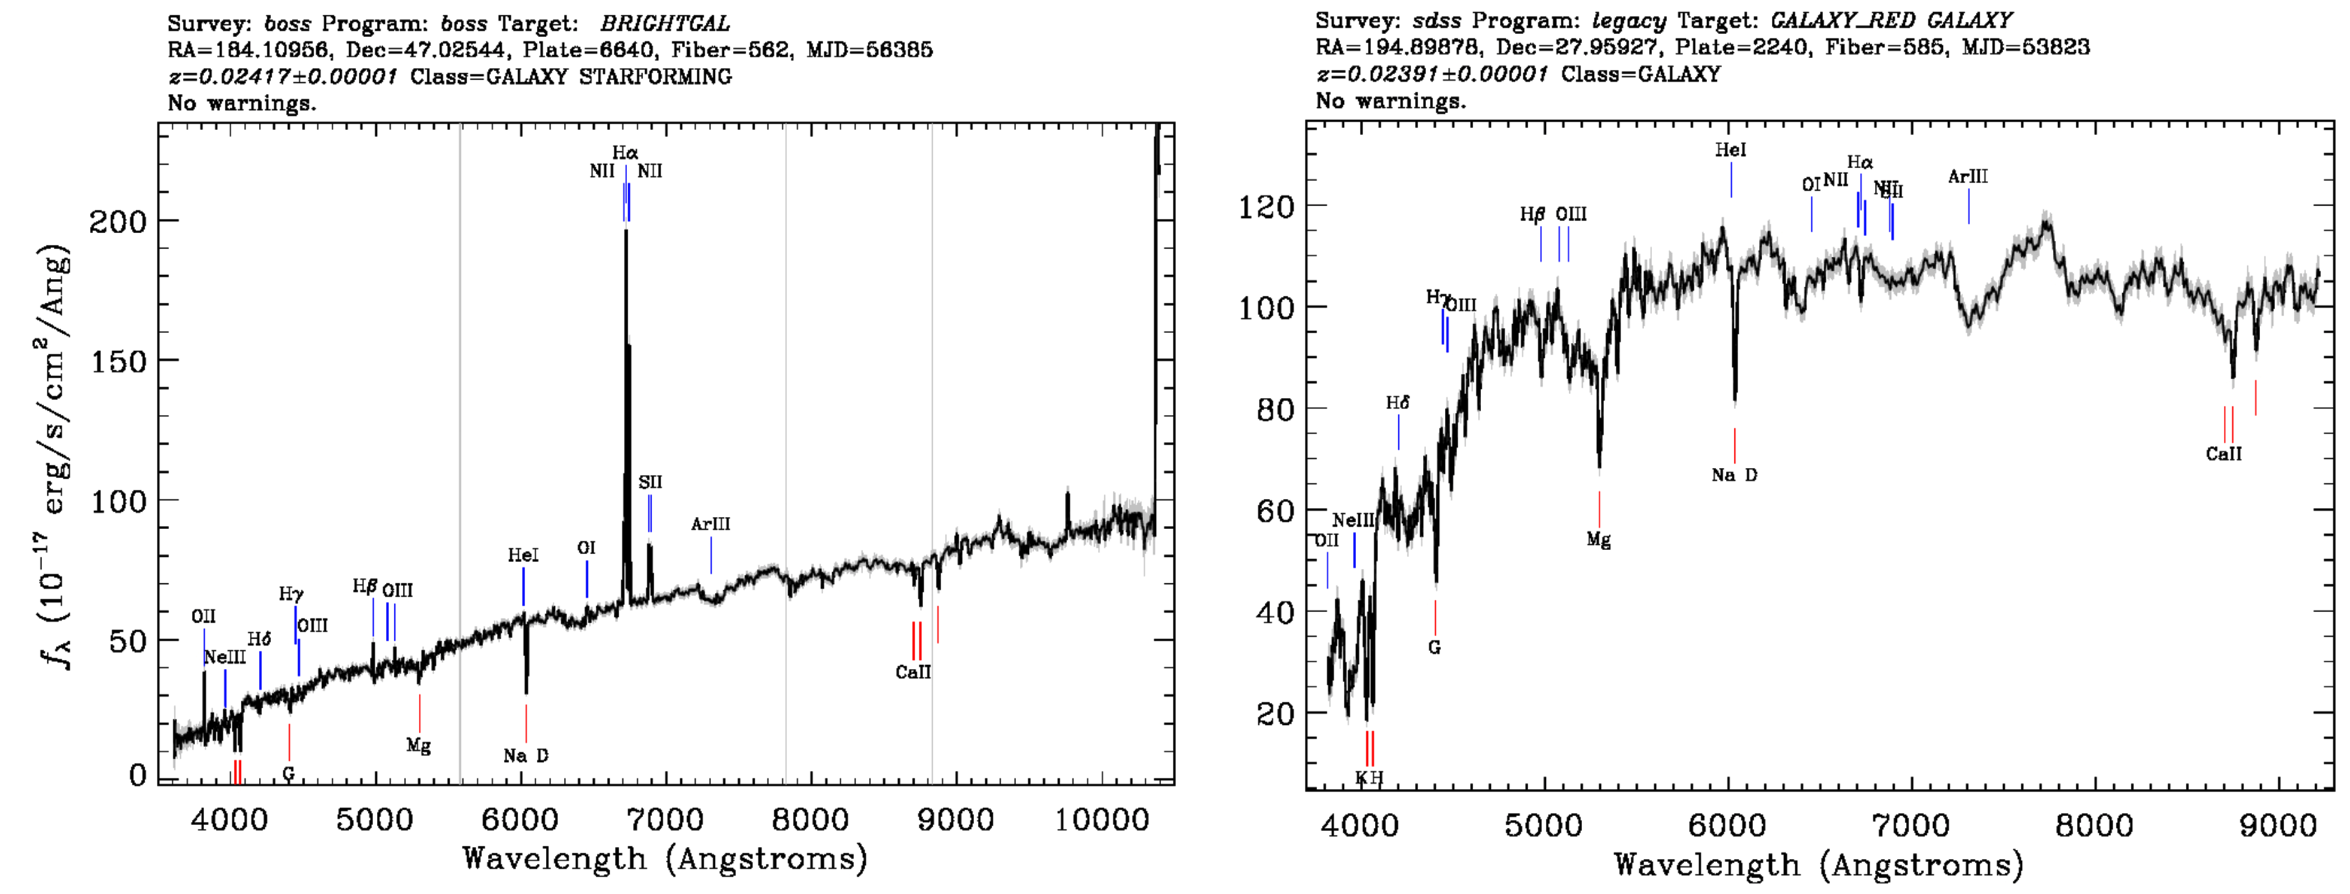
\includegraphics[width=0.99\textwidth]{../figures/04_hypergal/specgalsdss.png}
  \caption[Exemple de spectres de galaxies]{Exemple de spectres de
    galaxies (crédit SDSS). \textit{À gauche}, le spectre d'une galaxie
    spirale avec présence d'une forte raie d'émission
    $\text{H}_{\alpha}$. Cela se traduit par une forte présence d'étoiles
  jeunes (bleues) et de gaz qui favorise la formation stellaire. \textit{À droite},
le spectre d'une galaxie elliptique. On peut remarquer d'une part
l'abscence de raie d'émission $\text{H}_{\alpha}$, d'autre part une
forte perte en flux vers $4000$\AA. Cela trahit la très faible présence
d'étoiles jeunes (bleues) dans la galaxie et un faible taux de formation
stellaire.}
  \label{fig:specgalsdss}
\end{figure}

Modéliser une SED galactique revient donc à comprendre chacune de ces
interactions et leur répercussions.

Malgrès tout, certaines corrélations entre plusieurs paramètres rendent cette tâche
très difficile, comme par exemple la dégénerescence entre l'âge et la
métallicité \citep{Worthey}, ou encore l'âge et l'atténuation
\citep{Papovich}.

Ces deux dernières décennies ont été extrêmement riches en développement de modèles
et observations panchromatiques, permettant une compréhension de plus en
plus fine de la formation et l'évolution d'une galaxie.

Ont vu ainsi le jour des modèles de populations stellaires grâce à
\citet{Fioc1997}, \citet{BruzualCharlot2003} et \citet{Maraston2005}.
D'un autre côté, différentes lois d'atténuation par la poussière ont été
développées, comme par \citet{Calzetti1994,Calzetti2000} via l'étude de SED de
galaxies proches ayant un fort taux de formation stellaire, ou encore
avec une approche plus théorique de modèles de transferts radiatifs
\citep{WittGordon}.
Comme mentionné précédemment, la poussière ré-émet dans l'infrarouge et
l'étude et la modélisation de ce phénomène est un domaine actif de
recherche \citep{Casey2012, Dale2014, Draine2007, CharyElbaz}.

La manipulation de modèles pour chaque processus physique en oeuvre dans
une galaxie a permis l'émergence de nombreuses méthodes pour fitter une
SED. Ces nouvelles techniques permettent ainsi d'inférer les propriétés intrinsèques des galaxies
observées (locales, globales ou les deux), de pouvoir interpoler un
spectre à partir d'informations photométriques ou encore d'en estimer le
redshift.

\subsection{SED Fitter}

Le fit d'une distribution énergétique spectrale d'une galaxie est la
méthode première permettant d'inférer ses propriétés physiques intrinsèques à
partir d'observations. Ces propriétés peuvent ensuite être confrontés
aux prédictions provenant de théories d'évolution et formations de
galaxies. De ce fait, l'utilisation de SED Fitter est une pratique très
fréquente
lorsqu'il s'agit de tester des hypothèses en astronomie extragalactique
\citep{Tinsley1980, Walcher2011, Conroy2013, Chevallard2016, Briday22}. 

Trois composantes sont nécessaires pour procéder à un fit de SED : un
modèle physique qui décrit les différentes contributions qui la
composent, des données d'observations de la galaxie (photométriques
et/ou spectroscopiques) et le fitteur lui-même qui va inférer la
combinaison adéquate entre les modèles physiques et les observations.

De nombreuses techniques de SED Fitting ont été développées, certaines
basées sur 
la simple optimisation de maximum de vraisemblance, parfois appelée code
d'inversion, comme dans \pkg{ULySS}\footnote{\url{http://ulyss.univ-lyon1.fr}}\citep{KolevaUlyss}, \pkg{FIREFLY}\footnote{\url{http://www.icg.port.ac.uk/firefly/}}
\citep{WilkinsonFirefly} ou \pkg{LEPHARE}\footnote{\url{https://www.cfht.hawaii.edu/~arnouts/LEPHARE/lephare.html}} \citep{ArnoutsLephare} plus
axé sur la détermination de redshift photométrique.

Cette technique est très populaire de part sa rapidité de calcul et une
certaine simplicité à mettre en place. Néanmoins ces avantages sont
bridés par certaines limites. Par exemple, de part la haute
non-Gaussianité de certains espaces de vraisemblance, un léger changement
dans les données d'entrées (comme un bruit dans une image photométrique
de galaxie) peut conduire à de grands écarts dans les paramètres
inférés \citep{Ocvirk}.
Par ailleurs, une méthode de maximum de vraisemblance peut être diffcile à adapter
à des modèles hautement non-linéaires comme l'émission par la poussière.

Dans l'optique de résoudre ces problèmes, des techniques de forward-modeling
Bayesien ont à leur tour été développées. Avec cette méthode, des
grilles de paramètres sont pré-calculées puis comparées aux
observations. Le calcul de vraisemblance est alors très rapidement
déterminée, malgrés le fait que le nombre de modèle à calculer au
préalable croît exponentiellement à mesure que l'on rajoute des
paramètres. Parmi les codes développés à partir de cette méthode, on peut citer \citet{Kauffman2003}, \citet{Salim2007}, le
framework \pkg{CIGALE}\footnote{\url{https://cigale.lam.fr}}
\citep{Burgarella2005, Noll2009, Boquien2019} ou encore
\pkg{MAGPHYS}\footnote{\url{http://www.iap.fr/magphys/}}
\citep{Cunha2008MAGPHYS}.

Le succès du forward-modeling Bayesien a rapidement été adopté, et
étendu à un couplage avec des algorithmes de Monte-Carlo par chaînes de
Markov (MCMC) pour plus efficacement explorer l'espace des
posterior. Cette extension, initiée par \citet{Acquaviva2011} avec
\pkg{GalMC} (retiré du domaine public par faut de maintenance), puis
rapidement suivi de codes plus récents tels que
\pkg{BEAGLE}\footnote{\url{http://www.jacopochevallard.org/beagle/}}
\citep{Chevallard2016},
\pkg{BAGPIPES}\footnote{\url{https://github.com/ACCarnall/bagpipes}}
\citep{Carnall2018, Carnall2019} ou encore plus récemment
\pkg{Prospector}\footnote{\url{https://github.com/bd-j/prospector}}
\citep{JohnsonProspector} et
\pkg{piXedfit}\footnote{\url{https://github.com/aabdurrouf/piXedfit}}
\citep{Abdurro'ufPixedfit}.

Nous terminerons la présentation des SED Fitter en mentionnant le site
\url{sedfitting.org}, maintenu par Tamas Budavari, Daniel Dale, Brent
Groves et Jakob Walcher qui regroupe la grande majorité des codes et set
de modèles disponibles publiquement.

\section{Présentation du Pipeline}\label{sec:pipeline}
%\label{sec:xxx}

\begin{figure}
  \centering
  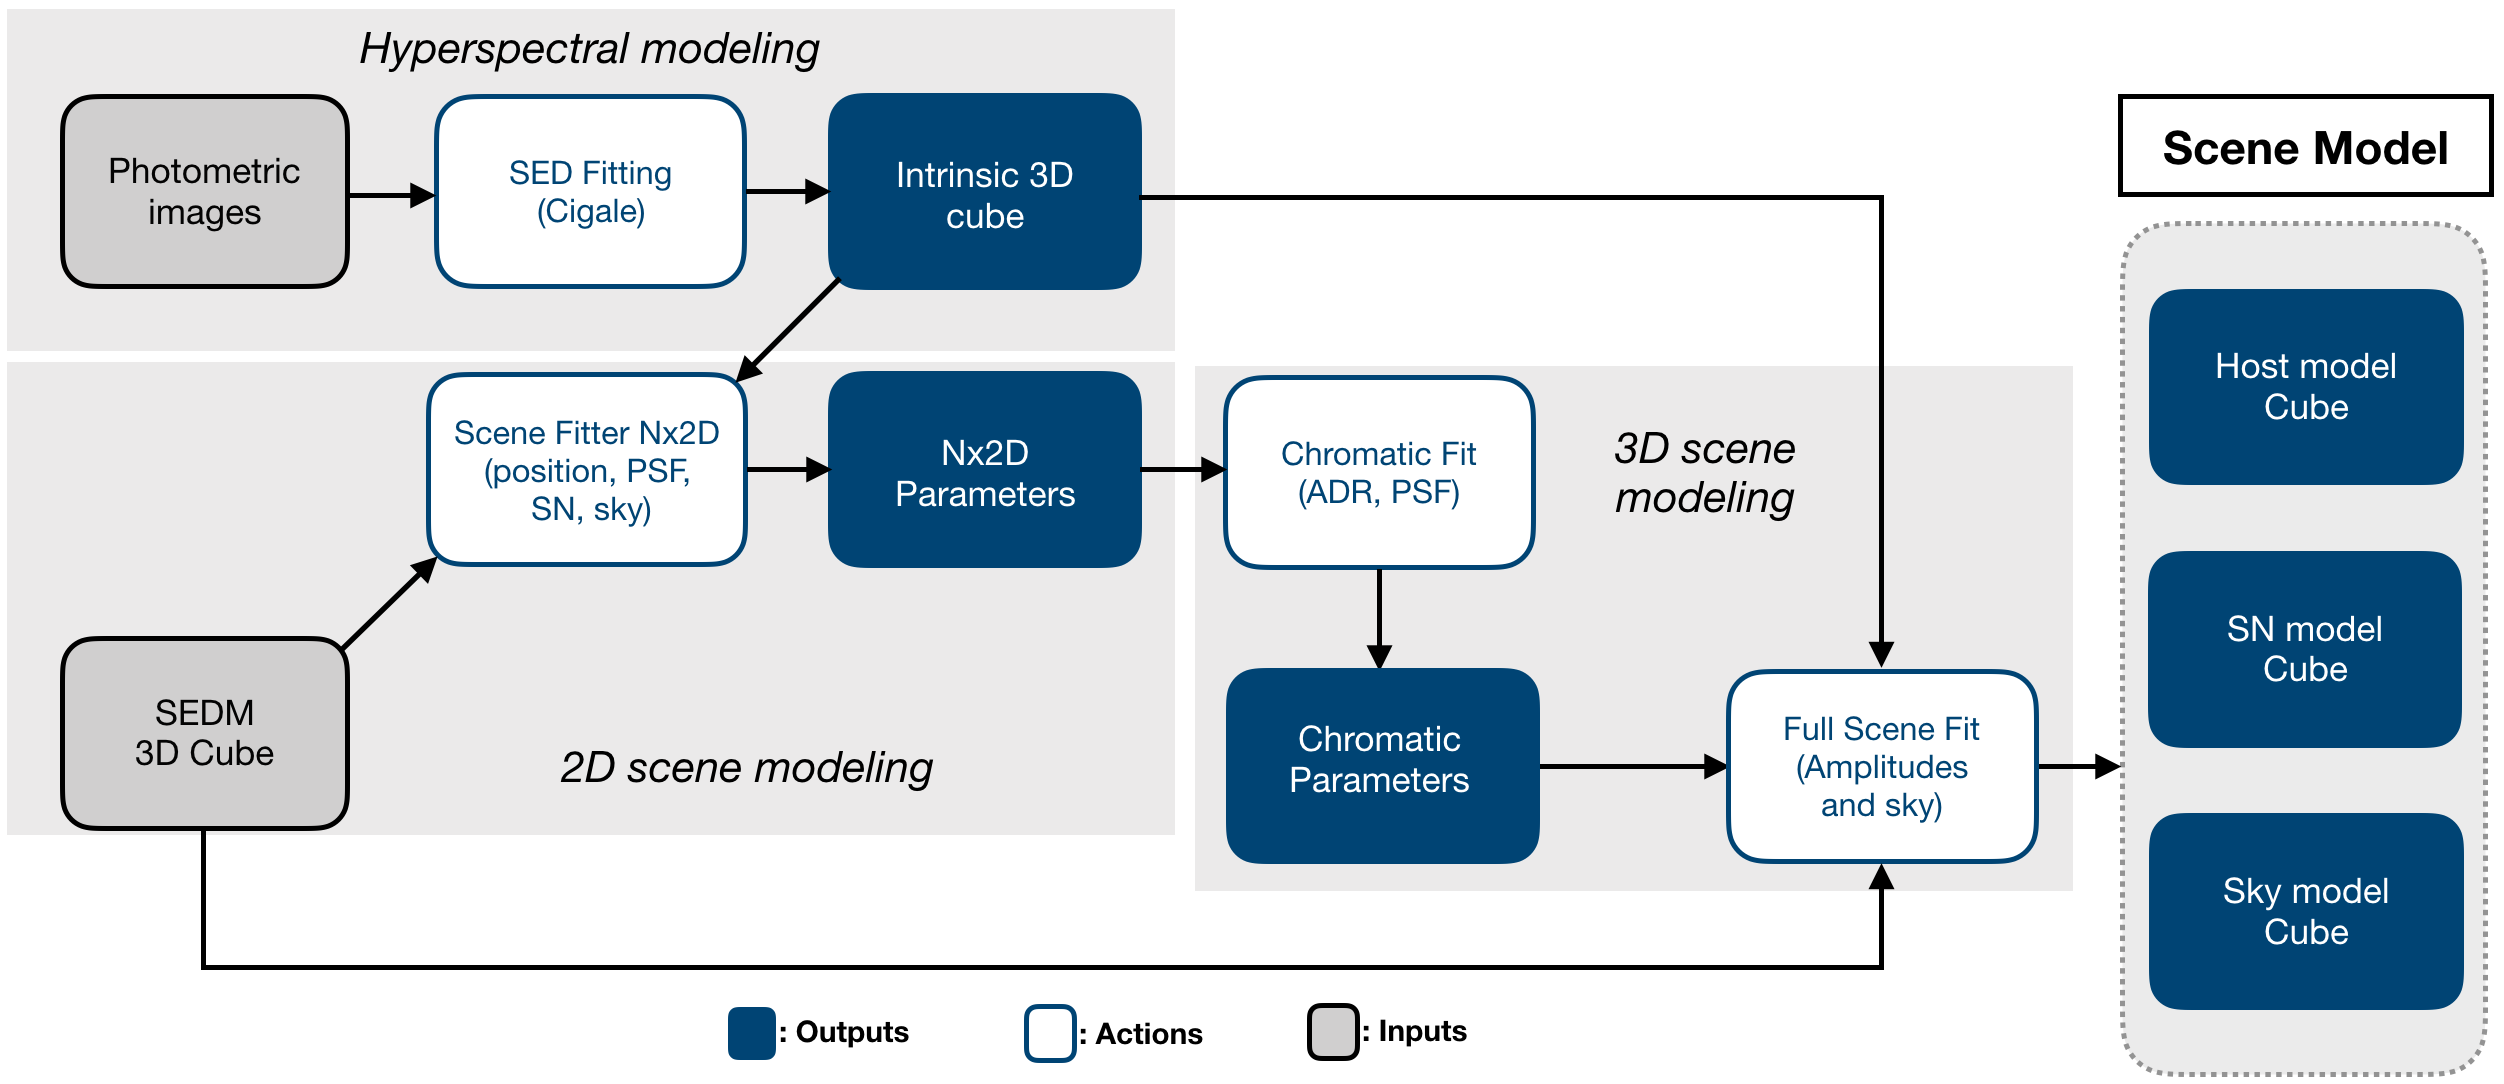
\includegraphics[width=0.99\textwidth]{../figures/04_hypergal/softdaghypergal.png}
  \caption[Présentation du pipeline \hypergal]{Présentation du pipeline \hypergal.}
  \label{fig:softdaghypergal}
\end{figure}

Nous allons à présent introduire le modéliseur de scène \hypergal.
Les étapes principales de ce pipeline sont présentées dans la
Figure~\ref{fig:softdaghypergal}, et tracerons l'organisation de cette
Partie du manuscrit.

\subsection{Cube intrinsèque}

Comme abordé dans la section~\ref{sec:ideahypergal}, le coeur
d'\hypergal repose sur la conception d'un cube 3D contenant la galaxie
hôte isolée de sa supernova: c'est la modélisation hyperspectrale de la galaxie. Le but n'est pas de remonter aux propriétés
intrinsèques de la galaxie, mais de simplement être en mesure
d'interpoler un spectre cohérent à l'échelle local.

Cette étape, entièrement indépendante des observations de la
SEDm, va nécessiter l'utilisation d'un SED Fitter, que nous avons
introduit dans la section~\ref{sec:sedfitting}. Dans un premier temps,
nous allons 
récupérer des images de différentes bandes photométriques de la galaxie hôte de la supernova
détectée par ZTF. On procèdera ensuite à un fitting de SEDs de portions
locales de la galaxie, ce qui permettra d'obtenir une multitude de
spectres propre à chaque région de la galaxie. Avec un échantillonnage spectral
adéquat, nous serons ainsi en mesure de reconstruire un cube 3D, dont
les deux dimensions spatiales ($x$, $y$) seront définis par les images
photométriques, et la dimension spectral par le SED Fitter. Le cube
résultant ne contiendra ainsi que la galaxie hôte, et sera appelé dans
la suite de ce manuscrit \textit{cube intrinsèque}. Cette étape de
modélisation hyperspectrale est détaillée dans le Chapitre~\ref{ch:modelhyperspec}.

\subsection{Modélisation de scène 2D}

Dans cette seconde étape, les observations de la SEDm deviennent
nécessaires: le but ici est de projeter le cube intrinsèque de la
galaxie dans l'espace des observations. Pour faire cela, nous allons de
façon indépendante caractériser la réponse impulsionnelle spatiale et
spectrale de la SEDm (Chapitre~\ref{ch:irf}).

En utilisant ces informations, nous projetterons dans l'espace de la
SEDm le cube intrinsèque préalablement scindé en $N$ méta-tranches
(2D). Il faudra pour cela prendre en compte la forme et la taille de l'échantillonnage
spatial des deux espaces (source photométrique et MLA de la SEDm) ainsi que la différence de seeing.
En plus de la composante galactique, nous caractériserons les composantes
de supernova, de fond de ciel et de potentiels artefacts à modéliser
pour compléter la scène.
La projection de chaque meta-tranche dans l'espace SEDm sera fittée aux
meta-tranches correspondantes de l'observation, dont la minimisation permettra de récupérer un set de
$N\times2D$ paramètres.

\subsection{Modélisation chromatique et projection 3D}

Les $N\times2D$ paramètres sont ensuite utilisés pour fixer la chromaticité des composantes de la scène, comme la réponse impulsionnelle
spatiale de la SEDm (fonction d'étalement de point; PSF) ou la
variation de la position des objets dans le MLA due à la réfraction de
la lumière par l'atmosphère (ADR). Les modèles de chromaticités sont
déterminés a priori, et les paramètres de ces modèles sont fittés à
partir des $N\times2D$ paramètres obtenus de l'étape précédente.

Une fois la chromaticité fixée, l'ensemble des paramètres de projection de chaque tranche
du cube intrinsèque dans l'espace SEDm devient fixe, et seuls les
paramètres d'amplitudes (fond de ciel, supernova...) sont fittés pour
chaque longueur d'onde. Cette étape permet ainsi d'extraire les trois
composantes de la scène d'observation de la SEDm, à savoir le background, la galaxie hôte et la
source ponctuelle.

%\bibliographystyle{../main/aa_url}
%\bibliography{99_references}
\end{document}

%%% Local Variables:
%%% mode: latex
%%% TeX-master: t
%%% End:
